\documentclass[a4paper,12pt]{article}
\usepackage[margin=2cm]{geometry}

% Pacchetti utili di base
\usepackage[utf8]{inputenc}   % codifica dei caratteri
\usepackage[T1]{fontenc}      % font encoding
\usepackage[italian]{babel}   % lingua italiana
\usepackage{graphicx}         % immagini
\usepackage{hyperref}         % link cliccabili
\usepackage{amsmath}          % align center
\usepackage{listings}         %codice programmazione
\usepackage{xcolor}           % per colori opzionali del codice
\usepackage{float}     % permette [H]
\usepackage{algorithm}
\usepackage{algpseudocode}
\usepackage{amsmath}
\usepackage{amssymb}
\usepackage[most]{tcolorbox}
\usepackage{cancel}

% Informazioni sul documento
\title{Algebra numerica}
\author{Nicolò Giuliani}
\date{}
\begin{document}
\maketitle
\tableofcontents   % <-- genera automaticamente la pagina dell'indice
\newpage 
\section{Zeri di funzione}
\subsection{Metodo di bisezione}
Dato un $a,b \in D$ tale che $f(a) < 0, f(b) > 0$: \\
\vspace{1em} Prendiamo in considerazione gli intervalli
\begin{align*}
    I_k = [a_k, b_k] \\
    I_k \subset I_{k+1} \subset \dots \subset I_1 
\end{align*}
con $f(a_k)f(b_k) < 0$:
\begin{align*}
    \boxed{f(c_k) = f(\frac{a_k+b_k}{2})}
\end{align*}
Tale che
\begin{align*}
    I_{k+1} = [a_k+1, b_k+1]= \begin{cases}
        [a_k, c_k] \text{ se } f(c_k) > 0 \\
        [c_k, a_k] \text{ se } f(c_k) < 0
    \end{cases}
\end{align*}
Fissato $\delta$ come tollerranza di errore possiamo calcolare il numero di iterazioni $k$
\begin{align*}
    k \geq \log_2\frac{b-a}{\delta}
\end{align*}
o per calcolare l'errore assoluto al passo $k$:
\begin{align*}
    E_a = \mid x_k - x^* \mid
\end{align*}
\begin{figure}[H]  % H = esattamente qui
    \centering
    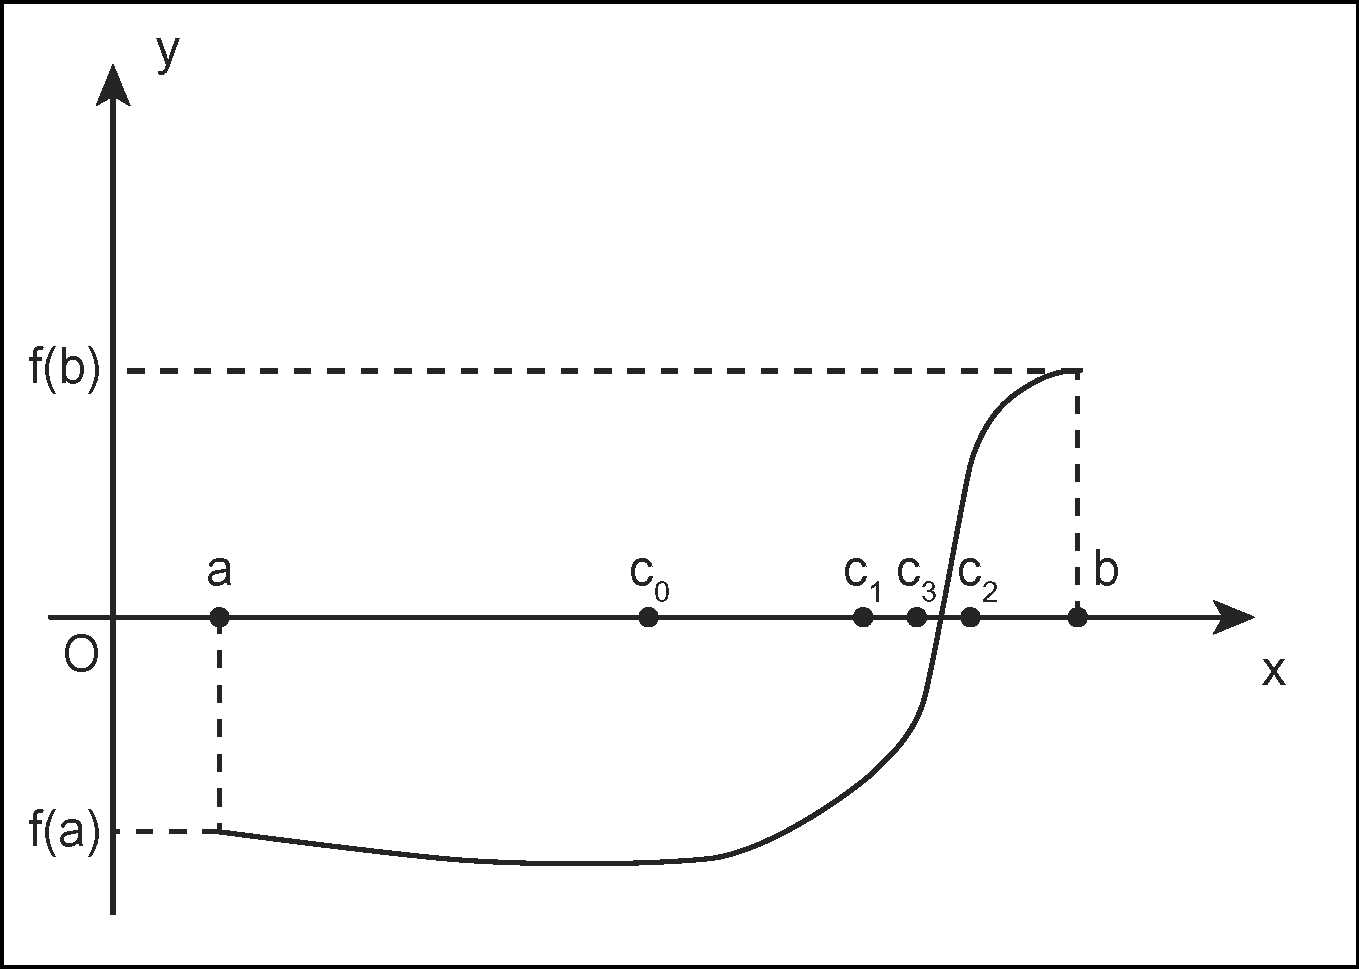
\includegraphics[width=0.6\textwidth]{img/bisezione.jpg}
    \caption{Esempio di esecuzione del metodo di punto fisso}
\end{figure}
\subsection{Metodo di punto fisso}
Per cercare $x^* \mid f(x^*) = 0$ possiamo cercare invece $x^* \mid g(x^*)=x^*$ tale che
\begin{align*}
    g(x)=x-f(x)\phi(x) \\
    \mid g'(x) \mid < 1\text{ vicino ad $x^*$} \\
    \rightarrow \text{ converge ad $x^*$}
\end{align*}
Iteriamo:
\begin{align*}
    x_{k+1} = g(x_k) \\
    \Rightarrow \boxed{x_{k+1} = x_k-f(x)\phi(x)}
\end{align*}
Possiamo approssimare con Taylor $x_0=x^*$
\begin{align*}
    g(x) = \sum_{n=0}^\infty \frac{g^{(n)}(x_0)}{n!}(x-x_0)^n \\
    \approx g(x^*) + g'(x^*)(x-x^*)+\frac{g''(x^*)}{2!}(x-x^*)^2 + \dots
\end{align*}
L'errore al passo $k$ lo definiamo come $e_k := |x_k - x^*|$
\begin{align*}
e_{k+1} &= |g(x_k) - x^*| \\
        &= |g(x_k) - g(x^*)| \\
        &= |g(x^*) + g'(x^*)(x_k-x^*) + \frac{g''(x^*)}{2!}(x_k-x^*)^2 + \dots - g(x^*)| \\
        &= |g'(x^*)(x_k-x^*) + \frac{g''(x^*)}{2!}(x_k-x^*)^2 + \dots| \\
        &= |g'(x^*) e_k + \frac{g''(x^*)}{2!} e_k^2 + \dots|
\end{align*}
Quindi approssimando possiamo dire 
\begin{align*}
    e_{k+1} \approx |g'(x^*)e_k + o(e_k)|
\end{align*}
L'errore si riduce proporzionalmente a $e_k$ $\rightarrow$ \textbf{convergenza lineare}.
\begin{figure}[H]  % H = esattamente qui
    \centering
    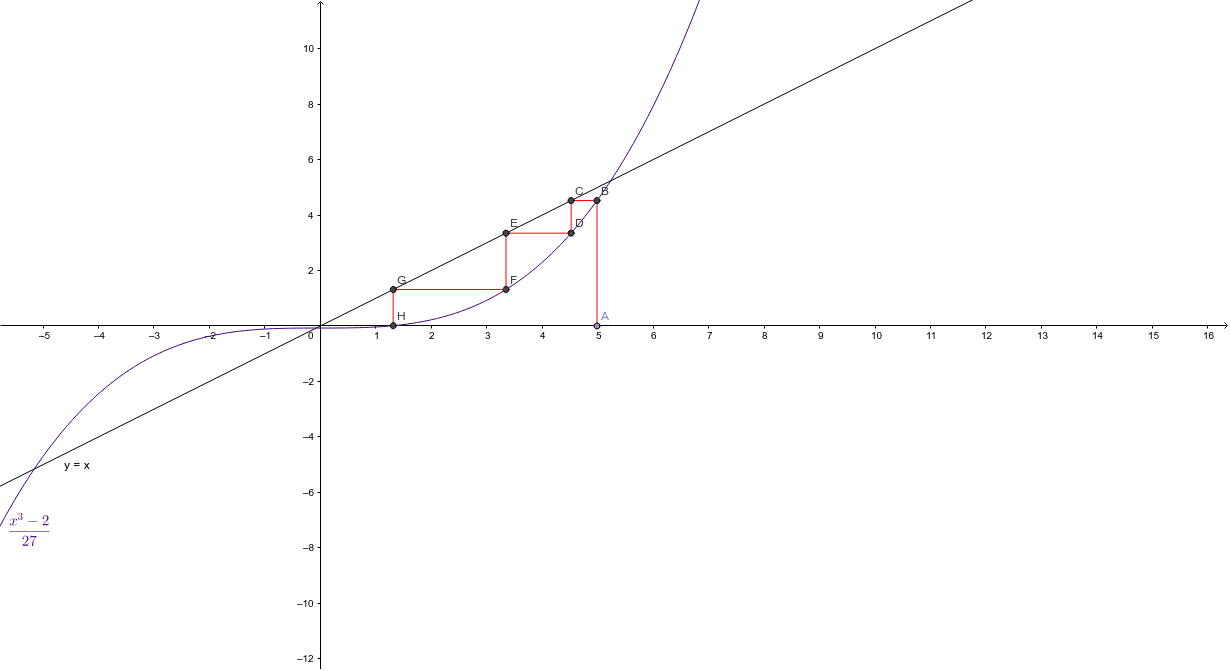
\includegraphics[width=0.9\textwidth]{img/punto_fisso.png}
    \caption{Esempio di esecuzione del metodo di bisezione}
\end{figure}
\subsection{Metodo di Newton}
Ora vediamo un caso speciale del punto fisso, se nell'algoritmo precendente abbiamo detto che
\begin{align*}
        e_{k+1} \approx |g'(x^*)e_k + \frac{g''(x^*)}{2!}(e_k)^2 |
\end{align*}
se
\begin{align*}
    0 < \mid g'(x) \mid < 1 \\
    e_{k+1} \approx |g'(x^*)e_k + o(e_k)|\\
    \rightarrow \text{Convergenza lineare}
\end{align*}
Quindi se prendiamo 
\begin{align*}
    \mid g'(x) \mid = 0 \\
    e_{k+1} \approx |\frac{g''(x^*)}{2!}(e_k)^2 + o(e_k^2)|\\
    e_{k+1} = C \cdot \mid e_k \mid^2 \quad \text{ con } C > 0\\
    \rightarrow \textbf{Convergenza quadratica}
\end{align*}
Per fare quello dobbiamo fare
\begin{align*}
    g'(x) = 0 = \frac{d}{dx}[x-f(x)\phi(x)] \\
    = 1 - f'(x)\phi(x) + \phi'(x)f(x) \\
\end{align*}
e dato che stiamo cercando $x^* \mid f(x^*)=0$:
\begin{align*}
    g'(x^*) = 1 - f'(x)\phi(x)
\end{align*}
e dato che $g'(x^*)=0$
\begin{align*}
    1-f'(x)\phi(x)=0\\
    \rightarrow \phi(x) = \frac{1}{f'(x)}
\end{align*}
Ricapitolando possiamo cercare
\begin{align*}
    g(x)=x-\frac{f(x)}{f'(x)}
\end{align*}
Ovvero algorimicamente possiamo iterare:
\begin{align*}
    \boxed{x_{k+1} = x_k-\frac{f(x_k)}{f'(x_k)}} 
\end{align*}
\begin{figure}[H]  % H = esattamente qui
    \centering
    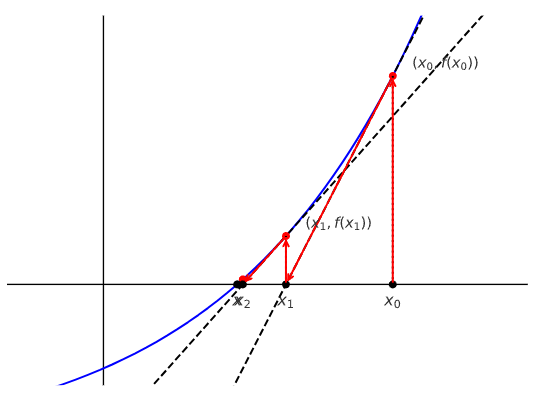
\includegraphics[width=0.5\textwidth]{img/newton.png}
    \caption{Esempio di esecuzione del metodo di Newton}
\end{figure}
\pagebreak
\section{Ottimizzazione}
Vogliamo trovare $x^* = \text{arg min}f(x)$.
\subsection{Metodo del gradiente}
\label{sec:met_grad}
Partendo dal metodo del punto fisso possiamo definire che vogliamo cercare $x \mid \nabla f(x)=0$:
\begin{align*}
    x_{k+1} = x_k-f(x_k)\phi(x_k) \\
\end{align*}
Definiamo per il punto fisso $f(x) = \nabla f(x_k)$:
\begin{align*}
        \Rightarrow  x_{k+1} = x_k - \nabla f(x_k) \phi(x_k)
\end{align*}
Dato che $\nabla f(x)$ indica la direzione di massima crescita noi prendiamo come direzione di ricerca la direzione di decrescita massima:
\begin{align*}
    p_k = - \nabla f(x_k)
\end{align*}
tale che
\begin{align*}
    p_k^T \nabla f(x_k) < 0 \\
    \Rightarrow - \nabla f(x_k)^T \nabla f(x_k) < 0 \\
    \Rightarrow \boxed{-\| \nabla f(x_k) \|_2^2 < 0}
\end{align*}
Quindi avremo 
\begin{align*}
    x_{k+1} = x_k + p_k \,\phi(x_k)
\end{align*}
Definiamo la funzione $\phi(x_k) = \alpha_k \in \mathbb{R}$. \\
Iteriamo con $\alpha_k > 0$ (\textit{step size})
\begin{align*}
    \boxed{x_{k+1} = x_k - \alpha_k \nabla f(x_k)}
\end{align*}
Dobbiamo stare attenti che $a_k$ ci permetta di discendere per la funzione:
\begin{align*}
    f(x_{k+1}) < f(x_k)
\end{align*}
Come scegliamo $a_k$?
\begin{itemize}
    \item $\forall k, \, \alpha_k = n \in R$ (statico)
    \item \textbf{Line search}
    \begin{itemize}
        \item Condizione di Armijo (costante di diminuzione del passo: $0<c<1$): \\
        \vspace{2em} garantisce che il passo $\alpha$ faccia diminuire sufficientemente la funzione
        \begin{align*}
            f(x_{k+1}) \leq f(x_k) - c \alpha (\nabla f(x_k))^T (\nabla f(x_k)) \\
            f(x_{k+1}) \leq f(x_k) \underbrace{- c \alpha \|\nabla f(x_k)\|^2}_{\text{\shortstack{diminuzione \\ minima accettabile}}}
        \end{align*}
        \item Tecnica di backtracking: \\
        dato un valore $\alpha = 1$ iniziale, riduciamo questo valore finche non troviamo un $\alpha_k$ che soddisfi condizione di Armijo.
            \begin{algorithm}[H]
            \caption{Tecnica di backtracking}
            \begin{algorithmic}[1]
            \State \textbf{Input:} $x_k$,$f()$,$\nabla f()$, $\alpha_0 > 0$, $c \in (0,1)$, $p \in (0,1)$
            \State $\alpha = \alpha_0$
            \Repeat
                \State $x_{k+1} = x_k - \alpha \nabla f(x_k)$
                \If{$f(x_{k+1}) > f(x_k) - c \alpha \|\nabla f(x_k)\|^2$}
                    \State $\alpha = p \alpha$
                \EndIf
            \Until{$f(x_{k+1}) \le f(x_k) - c \alpha \|\nabla f(x_k)\|^2$}
            \State \Return $\alpha$
            \end{algorithmic}
            \end{algorithm}

    \end{itemize}
\end{itemize}
Quindi nelle realta' implementiamo:
            \begin{algorithm}[H]
            \caption{Metodo del gradiente}
            \begin{algorithmic}[1]
            \State \textbf{Input:} $x_0$,$f()$,$\nabla f()$, $\alpha_0 > 0$, $c \in (0,1)$, $p \in (0,1)$
            \State $x_k = x_0$
            \For{($k=0; k< \text{max iter}; \, k\text{++}$)}
                \State $\alpha = $ backtracking($x_k, f(), \nabla f(), \alpha_0, c, p$)
                \State $x_{k+1} = x_k - \alpha \nabla f(x_k)$
            \EndFor
            \State \Return $x_{k+1}$
            \end{algorithmic}
            \end{algorithm}
\subsection{Metodo di Newton puro}
Dal metodo del gradiente sappiamo (a sua volta basato sul punto fisso):
\begin{align*}
      x_{k+1} = x_k - \nabla f(x_k) \phi(x_k) 
\end{align*}
Prendiamo $\phi(x) = H_f(x_k)^{-1}$
\begin{align*}
    x_{k+1} = x_k - \nabla f(x_k) H_f(x_k)^{-1}
\end{align*}
con $H_f(x_k)$ matrice Hessiana.\\
Quindi non iteriamo piu' con un passo statico o backtracking ma la hessiana misura la curvatura della funzione in tutte le direzioni in modo tale da modulare il passo:
\begin{itemize}
    \item Direzioni molto \textit{"ripide"} $\to$ passo più piccolo
    \item Direzioni piatte $\to$ passo più lungo
\end{itemize}
\begin{align*}
    \boxed{x_{k+1} = x_k - H_f(x_k)^{-1}\nabla f(x)}
\end{align*}
La funzione converge (quadraticamente) solo se $H_f(x_k)$ e':
\begin{itemize}
    \item Simmetrica: $A=A^T$
    \item \textbf{Definita positiva}: $\forall v\neq 0 \in \mathbb{R}^n: \, v^T A v>0$ o anche possiamo vedere se $\forall \lambda_A > 0$. 
\end{itemize}
Questo metodo cosi come e' non e' utilizzato perche' "troppo rognosa", esistono pero' delle varianti molto efficaci.
\subsection{Gradiente stocastico (SGD)}
Dato una funzione del tipo
\begin{align*}
    f(x) = \sum_{i=1}^N f_i(x)
\end{align*}
e vogliamo trovare $x^* = \text{arg min}f(x)$, avremo dunque bisogno del suo gradiente. Che puo' essere scritto anche come
\begin{align*}
    \nabla f(x) = \sum_{i=1}^N \nabla f_i(x)
\end{align*}
Con il SGD andiamo ad approssimare il gradiente originale con solo un set di dati della funzione completa.
\begin{align*}
    \nabla f(x) \approx \sum_{i \in \{i_1, \dots, i_m\}} \nabla f_i(x)
\end{align*}
Fissiato $m$ scelgo il \textbf{mini batch} $i_1,\dots,i_m$ ,o se $m=1$ il \textbf{batch}, casualmente \textbf{senza ripetizione} in $[1,N]$. \\
\vspace{2em}\\
Quindi potremo iterare nel metodo del gradiente
\begin{align*}
    x_{k+1} = x_k - \alpha_k \nabla f(x_k) \\
    \boxed{x_{k+1} \approx x_k - \alpha_k (\sum_{i \in \{i_1, \dots, i_m\}}f_i(x_k))}\\    
    = x_k - \alpha_k (\nabla f_{i_1}(x_k) + \dots + \nabla f_{i_m}(x_k))
\end{align*}
\textbf{Epoca}: Numero di iterazioni necessarie per aver utilizzato tutti gli $N$ dati del dataset almeno una volta.
\begin{align*}
    p = \frac{N}{m}
\end{align*}
Ovvero dopo $p$ iterazioni (usando $p$ mini-bach da $m$ dati ciascuno) tutti i dati da $1$ a $N$ sono stati utilizzati almeno 1 volta. \\
\vspace{1em}\\
Questo e' utile in IA per monitorare l'apprendimento (se dopo $p$ epoche il modello e' ancora stupido proviamo con $p+1$ epoche).
\pagebreak
\section{Approssimazione dei dati}
\label{sec:approssimazione}
Dato dei dati $\theta = (x_i,y_i)$ dobbiamo cerca una funzione coerente $f(\bar{x}; \theta)$ con $\bar{x} \in [min(x),max(x)]$.
\begin{figure}[H]  % H = esattamente qui
    \centering
    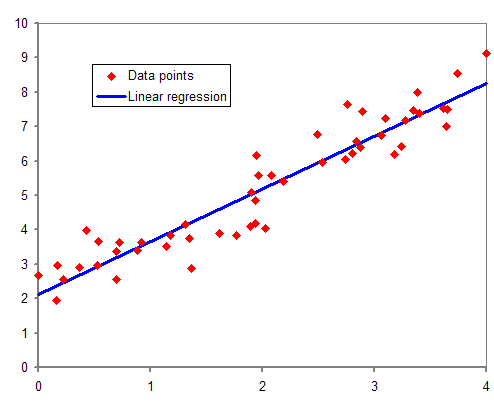
\includegraphics[width=0.6\textwidth]{img/reg.png}
\end{figure}
Per stabilire se una funzione sia piu' corente rispetto ad un altra dobbiamo avere una unita' di misura: \\
Definiamo la \textbf{loss function}
\begin{align*}
    \mathcal{L}(\theta) = \sum_{i=1}^n (f(x_i; \theta) - y_i)^2
\end{align*}
Ovvero dobbiamo trovare
\begin{align*}
    \min_\theta \,\mathcal{L}(\theta)
\end{align*}
La funzione basata sulla minimizzazione della perdita si chiama \textbf{regressione}.
\begin{itemize}
    \item $k=1$: $f(x; \theta) = \theta_0 + \theta_1x$ (pol. grado 1)
    \item $k=2$: $f(x; \theta) = \theta_0 + \theta_1x + \theta_2x^2$ (pol. grado 2)
    \item $k$: $f(x; \theta) = \theta_0 + \theta_1x + \theta_2x^2 + \dots + \theta_k x^k$ (pol. grado $k$)
\end{itemize}
Quindi la loss function per la regressione generale e':
\begin{align*}
    \mathcal{L}(\theta) = \sum_{i=1}^n (\theta_0 + \theta_1x + \theta_2x^2 + \dots + \theta_k x^k - y_i)^2
\end{align*}
Possiamo definire quindi:
\begin{itemize}
    \item $\theta = \begin{pmatrix}
        \theta_0 \\
        \theta_1 \\
        \theta_2 \\
        \vdots \\
        \theta_k
    \end{pmatrix}$
    \item $y = \begin{pmatrix}
        y_1 \\
        y_2 \\
        \vdots \\
        y_n
    \end{pmatrix}$
    \item Matrice $n \times k+1$ come:  
    $\Phi = \begin{pmatrix}
        x_1^0 && x_1^1 && \dots && x_1^k \\
        x_2^0 && x_2^1 && \dots && x_2^k \\
        \dots && \dots && \dots && \dots \\
        x_n^0 && x_n^1 && \dots && x_n^k \\
    \end{pmatrix}$
\end{itemize}
Allora definiamo la loss function:
\begin{align*}
    \mathcal{L} = \| \Phi \theta - y \|_2^2
\end{align*}
E per ottenere $\theta$ facciamo:
\begin{align*}
    \min_{\theta \in \mathbb{R}^{k+1}} \| \Phi \theta - y \|_2^2
\end{align*}
Questo e' chiamato \textbf{problema dei minimi quadrati (lineare)}.
\pagebreak
\section{Algebra lineare numerica}
\subsection{Norme vettoriali e matrici}
La distanza tra due vettori $x, y \in \mathbb{R}^n$ si calcola con:
\begin{itemize}
    \item Norma di Manhattan: $\| x-y \|_1 = \sum_{i=1}^n | x_i-y_i |$
    \item Norma euclidea: $\| x-y \|_2 = | \sqrt{\sum_{i=1}^n(x_i - y_i)^2} |$
    \item Norma del massimo: $\|x - y\|_\infty = \max_{1 \le i \le n} |x_i - y_i|$
\end{itemize}
Vediamo norme di matrice:
\begin{itemize}
    \item $\text{Norma 1 (matrice)}: \|A\|_1 = \max_j \sum_i |a_{ij}|$ 
    \item $\text{Norma 2 (matrice)}: \|A\|_2 = \sigma_{\max}(A)$
    \item $\text{Norma Frobenius}: \|A\|_F = \sqrt{\sum_{i,j} |a_{ij}|^2}$
\end{itemize}
\section{Sistemi lineari}
\begin{tcolorbox}[colback=blue!5!white, colframe=blue!75!black]
Definiamo $A$ invertibile se e solo se $dim(A)=rk(A)$. \\
$A$ invertibile = $A$ non singolare. \\
$A$ non invertibile = $A$ singolare.
\end{tcolorbox}
Dato 
\begin{align*}
    Ax = b \quad A \in \mathbb{R}^{n \times n}
\end{align*}
\begin{itemize}
    \item Il sistema ammette 1 sola soluzione $\forall b \in \mathbb{R}^n$ sse $A$ non e' singolare (= $A$ invertibile) $\iff det(A) \neq 0 \iff \exists A^{-1}$
    \begin{align*}
        Ax=b \\
        A^{-1}Ax = A^{-1} b \\
        \boxed{x = A^{-1} b}
    \end{align*}
    Questo vale solo se $A$ quadrata e invertibile. \\
    \textit{Nota}: Computazionalmente non si calcola $x=A^{-1}b$ perche' $O(n^3$). \\
    Se $A$ non e' quadrata facciamo \textbf{CGLS} (Conjugate Gradient)\label{sec:cgls}:
    \begin{align*}
        A^T A x = A^T b 
    \end{align*}
    Cosi avremo la matrice $A^T A$ quadrata e definita positiva (SPD).
    \item Algoritmi diretti per la soluzione: 
    \subsection{Fattorizzazione Cholesky}
    Per $A$ simmetrica ($A=A^T$) e definita positiva:
    \begin{align*}
        A=LL^T
    \end{align*}
    con 
    \begin{itemize}
        \item $L$ matrice singolare inferiore
        \item $L^T$ la sua transposta
    \end{itemize}
    \begin{align*}
        \begin{cases}
            Ly = b \\
            L^Tx=y
        \end{cases}    
    \end{align*}
    Costo computazionale: $O(\frac{1}{n^3})$. 
    \subsection{Fattorizzazione LU}
    Per $A$ quadrata:
\begin{tcolorbox}[colback=blue!5!white, colframe=blue!75!black]
Dando per scontato che definiamo:
\[
\begin{array}{c c}
\underbrace{
\begin{bmatrix}
 x & x & x & x \\
 0 & x & x & x \\
 0 & 0 & x & x \\
 0 & 0 & 0 & x
\end{bmatrix}}_{\text{matrice triangolare superiore}}
&
\begin{cases}
x_n = \frac{y_n}{t_{n,n}} \\
x_{n-1} = \frac{y_{n-1}- t_{n-1,n} x_n}{t_{n-1, n-1}} \\
x_{n-2} = \frac{y_{n-2}- t_{n-2,n-1} x_{n-1} - t_{n-2,n} x_n}{t_{n-2, n-2}} \\
\vdots  \\
x_1 = \dots
\end{cases}
\\[3em]
\underbrace{
\begin{bmatrix}
 x & 0 & 0 & 0 \\
 x & x & 0 & 0 \\
 x & x & x & 0 \\
 x & x & x & x
\end{bmatrix}}_{\text{matrice triangolare inferiore}}
&
x_i = \frac{y_i - \sum_{j=1}^{i-1}s_{ij}\cdot x_j}{s_{ii}}
\end{array}
\]

Per calcolarle (ognuna): $O\Big(\frac{n(n+1)}{2}\Big) = O\Big(\frac{n^2}{2}\Big)$
\end{tcolorbox}

Possiamo fattorizzare $A$:
\begin{align*}
    A = L \cdot U
\end{align*}
\begin{itemize}
    \item $L$ matrice triangolare inferiore con elementi uguale a 1 sulla diagonale
    \item $U$ matrice triangolare superiore
\end{itemize}
\begin{align*}
    Ax=b \\
    L\cdot \underbrace{U \, x}_y = b \\
    \boxed{\begin{cases}
        Ly=b \\
        Ux=y
    \end{cases} }
    \rightarrow
    \begin{cases}
        O(\frac{n^2}{2}) \\
        O(\frac{n^2}{2})
    \end{cases}
    = O(n^2)
\end{align*}
Esecuzione: \\

\[
A = 
\begin{bmatrix}
a_{11} & a_{12} & \dots & a_{1n} \\
a_{21} & a_{22} & \dots & a_{2n} \\
\vdots & \vdots & \ddots & \vdots \\
a_{n1} & a_{n2} & \dots & a_{nn}
\end{bmatrix}
\]

\textbf{Step 1: Eliminazione della prima colonna}

Definiamo i coefficienti:

\[
e_{i1} = -\frac{a_{i1}}{a_{11}}, \quad i = 2, \dots, n
\]

e la matrice elementare:

\[
E_1 =
\begin{bmatrix}
1 & 0 & \dots & 0 \\
e_{21} & 1 & \dots & 0 \\
\vdots & \vdots & \ddots & \vdots \\
e_{n1} & 0 & \dots & 1
\end{bmatrix}
=
\begin{bmatrix}
1 & 0 & \dots & 0 \\
-\frac{a_{21}}{a_{11}} & 1 & \dots & 0 \\
\vdots & \vdots & \ddots & \vdots \\
-\frac{a_{n1}}{a_{11}} & 0 & \dots & 1
\end{bmatrix}
\]

Applichiamo \(E_1\) a \(A\) per ottenere:

\[
A_2 = E_1 A =
\begin{bmatrix}
a_{11} & a_{12} & \dots & a_{1n} \\
0 & a_{22}^{(2)} & \dots & a_{2n}^{(2)} \\
\vdots & \vdots & \ddots & \vdots \\
0 & a_{n2}^{(2)} & \dots & a_{nn}^{(2)}
\end{bmatrix}
\]

---

\textbf{Step \(k\): Eliminazione della colonna \(k\)}

In generale, al passo \(k\) definiamo:

\[
e_{ik} = -\frac{a_{ik}^{(k)}}{a_{kk}^{(k)}}, \quad i = k+1, \dots, n
\]

e la matrice elementare:

\[
E_k =
\begin{bmatrix}
I_{k-1} & 0 \\
0 & \tilde{E}_k
\end{bmatrix}, \quad
\tilde{E}_k =
\begin{bmatrix}
1 & 0 & \dots & 0 \\
e_{k+1,k} & 1 & \dots & 0 \\
\vdots & \vdots & \ddots & \vdots \\
e_{nk} & 0 & \dots & 1
\end{bmatrix}
\]

Dove \(I_{k-1}\) è l'identità di dimensione \((k-1)\times(k-1)\).  
Applicando \(E_k\) alla matrice aggiornata \(A_k\) otteniamo:

\[
A_{k+1} = E_k A_k =
\begin{bmatrix}
* & * & \dots & * \\
0 & * & \dots & * \\
\vdots & \vdots & \ddots & \vdots \\
0 & 0 & \dots & *
\end{bmatrix}
\]
Costo al passo $k$: $O((n-k)^2)$. \\
Costo totale $E_1,\dots,E_k$: $\sum_{i=1}^{n-1} O(i^2) \approx O(\frac{n^3}{3})$. \\
\vspace{1em}\\
Ripetendo questo procedimento fino a \(k = n-1\), otteniamo la matrice triangolare superiore \(U\):

\[
U = E_{n-1} \dots E_1 A
\]
Ogni matrice $E_k$ e' invertibile e si puo' scrivere:
\begin{align*}
    A=E_1^{-1}E_2^{-1}\dots E_{n-1}^{-1} U 
\end{align*}
Definiamo $L = E_1^{-1}E_2^{-1}\dots E_{n-1}^{-1}$
\begin{align*}
    \rightarrow A = LU
\end{align*}
con $L$ triangolare inferiore con diagonale 1, $U$ triangolare superiore.
\end{itemize}
Il costo computazionale della fattorizzazione LU e' $O(\frac{2n^3}{3}) + \cancel{2O(\frac{n^2}{2})}$. \\
\vspace{2em}\\
\subsection*{Tutte le matrici non singolari posso essere fattorizzate LU?}
Prendiamo in considerazione
\begin{align*}
    A =\begin{pmatrix}
        0 & 1 & 2 \\
        3 & 4 & 5 \\
        6 & 7 & 8
    \end{pmatrix}
\end{align*}
Dobbiamo calcolare $L$:
\begin{align*}
    L = \begin{pmatrix}
        1 & 0 & 0 \\
        x & 1 & 0 \\
        x & x & 1
    \end{pmatrix}
\end{align*}
Quindi calcoliamo le matrici elementari per poi avere $L$, partiamo con $E_1$:
\begin{align*}
    e_{11} = -\frac{a_{11}}{a_{11}} = - \frac{0}{0} \\
    \to \text{Impossibile}
\end{align*}
$\rightarrow$ Non possiamo fattorizzare $A$ con $LU$! 
\vspace{1em}
\subsection*{Modifica algoritmo LU: Permutazione}
\textit{Idea}: ad ogni passo $k$ prima di calcolare $E_k$ scambio le righe di $A_k$ tale che
\begin{align*}
    a_{kk} = \max_{i=k,\dots,n} \{(a_{i, k})\}
\end{align*}
Esempio: riprendiamo in considerazione la matrice $A$ di prima
\begin{align*}
        A =\begin{pmatrix}
        0 & 1 & 2 \\
        3 & 4 & 5 \\
        6 & 7 & 8
    \end{pmatrix}
\end{align*}
Definiamo $P_1$ la matrice di \textbf{permutazione} (derivante da $I$ scambiando le righe):
\begin{align*}
    P_1 = \begin{pmatrix}
        0 & 0 & 1 \\
        0 & 1 & 0 \\
        1 & 0 & 0
    \end{pmatrix}
\end{align*}
Allora attraverso il prodotto
\begin{align*}
    A_0 = P_1 A = \begin{pmatrix}
        6 & 7 & 8 \\
        3 & 4 & 5 \\
        0 & 1 & 2
    \end{pmatrix}
\end{align*}
E ora applichiamo $LU$ normalmente:
\begin{align*}
    E_1 = \begin{pmatrix}
        x & x & x \\
        0 & x & x \\
        0 & x & x
    \end{pmatrix}
\end{align*}
\begin{align*}
    A_1 = E_1 A_0
\end{align*}
E poi riapplichiamo $a_{22} = \max_{i=2,\dots,n} \{(a_{i, 2})\}$, e cosi' via. \\
\vspace{5px} \\
Questo algormito che abbiamo applicato alla matrice $A$ si chiama fattorizzazione 
\begin{align*}
    P \cdot A = L \cdot U
\end{align*}
In soldoni:
\begin{align*}
    Ax=b \\
    PAx=Pb \\
    LUx = Pb 
\end{align*}
\begin{align*}
    \rightarrow \boxed{\begin{cases}
        Ly = P b \\
        Ux = y
    \end{cases}}
\end{align*}
\textit{Definizione}: Se $A$ e' non singolare ($n\times n$) allora esistono:
\begin{itemize}
    \item $P$ matrice di permutazione
    \item $L$ matrice triangolare inferiore con 1 sulla diagonale 
    \item $U$ matrice triangolare superiore
\end{itemize}
tali che 
\begin{align*}
    PA = LU
\end{align*}
Questo algoritmo e' \textbf{stabile}! (erorre alg. limitato)
\vspace{2em}\\
\subsection{Condizionamento}
\begin{tcolorbox}[colback=orange!5!white, colframe=orange!75!black, title = Teorema Rouchè Capelli]
Dato $A \in \mathbb{R}^{m \times n}, x \in \mathbb{R}^n, b \in \mathbb{R}^m$:\\
\begin{itemize}
    \item Il sistema lineare $Ax=b$ ammette soluzione unica se $rk(A)=rk(A | b)=n$
    \item Il sistema $Ax=b$ ha infinite soluzioni se $rk(A) = rk(A|b) < n$
    \item Il sistema $Ax=b$ non ha soluzioni se $rk(A) \neq rk(A|b)$
\end{itemize}
Possiamo anche \textit{semplificarlo} come 
\begin{itemize}
    \item Se $m = n$ e le equazioni sono indipendenti $\Rightarrow$ soluzione unica.
    \item Se $m < n$ (sottodeterminato) $\Rightarrow$ infinite soluzioni possibili se compatibile.
    \item Se $m > n$ (sovradeterminato) $\Rightarrow$ generalmente nessuna soluzione.
\end{itemize}
\end{tcolorbox}
Dato un sistema di dati in input $(A,b)$ e il rispettivo output $x=A^{-1}b$ se viene aggiunto un \textbf{errore sui dati} $(\Delta A, \Delta b)$:
\begin{align*}
(A,b) &\xrightarrow{A^{-1}} x \\
(A+\Delta A,\,b+\Delta b) &\xrightarrow{(A+\Delta A)^{-1}} x + \Delta x
\end{align*}

Ma se nel nostro modello predittivo otteniamo un errore risultato maggiore dell'errore sui dati previsto
\begin{align*}
    \| \Delta x \| >> \| \Delta A, \Delta b \|
\end{align*}
abbiamo un modello inesatto.\\
\vspace{1em}\\
Sia $x^*$ soluzione del sistema $Ax=b$, cerchiamo la soluzione $\tilde{x}$ del sistema perturbato:
\begin{align*}
    (A+\Delta A)\tilde{x} = b + \Delta bx
\end{align*}
Esempio:
\begin{align*}
        A=\begin{pmatrix}
        1 & 2 \\
        0.4999 & 1.001
    \end{pmatrix} \quad (b+\Delta b) = \begin{pmatrix}
        3 \\ 1.5
    \end{pmatrix}
\end{align*}
Soluzione reale: $\Delta A= \begin{pmatrix}
    0 \\ 0
\end{pmatrix}, \quad \Delta b = \begin{pmatrix}
    0 \\0
\end{pmatrix}$
\begin{align*}
    \begin{cases}
        1x_1^* + 2x_2^* = 3 \\
        0.4999x_1^* + 1.001x_2^* = 1.5
    \end{cases} \\
    \rightarrow \begin{cases}
        x_1^* = 1 \\
        x_2^* = 1
    \end{cases}
\end{align*}
Soluzione del sistema perturbato: $\Delta A = \begin{pmatrix}
    0.1 \\
    0.1
\end{pmatrix}, \quad \Delta b = \begin{pmatrix}
    0 \\0
\end{pmatrix}$
\begin{align*}
    \begin{cases}
        1\tilde{x_1} + 2\tilde{x_2} = 3 \\
        0.5\tilde{x_1} + 1.002\tilde{x_2} = 1.5
    \end{cases} \\
    \rightarrow \begin{cases}
        \tilde{x_1}= 3 \\
        \tilde{x_2} = 0
    \end{cases}
\end{align*}
Notiamo come per un minusco incrementio SOLO per $\Delta A$ il risultato sia completamente sballato! \\
Infatti una piccola differenza nella matrice come $\Delta A$
\begin{align*}
    \frac{\| \Delta A\|}{\| A \|} \approx 5.7 \cdot 10^{-4}
\end{align*}
Porta un grande cambiamento nella soluzione
\begin{align*}
    \frac{\| \tilde{x}-x^* \|}{\| x^* \|} \approx 1.58
\end{align*}
I problemi che soffrono di grandi perturbazioni nei risultati per colpa di piccole perturbazioni nei dati sono definiti \textbf{mal condizionati}.
\subsection{Problema minimi quadrati e SVD}
\label{sec:min_quad}
Possiamo risolvere $Ax=b$ attraverso il \textbf{metodo dei minimi quadrati}
\begin{align*}
    \min_x \|Ax-b \|_2^2 \\
    \Rightarrow f(x) = \|Ax-b \|_2^2 \\
    \Rightarrow f(x) = (Ax-b)^T(Ax-b) \\
\end{align*}
Noi cerchiamo $x \mid \nabla f(x)=0$:
\begin{align*}
        \frac{d}{dx}[(Ax-b)^2(Ax-b)] = 0 \\
        \Rightarrow
        \boxed{A^T A x = A^T b}
\end{align*}
Cosi avremo una matrice quadrata e definita positiva (SPD)! \\
Costo computazionale tramite equazioni normali: $O(mn^2 + n^3)$. \\ 
\vspace{1px}\\
Potremmo anche risolverlo con \textbf{Cholesky} + LU: $O(mn^2 + \frac{1}{3}n^3)$
\begin{tcolorbox}[colback=blue!5!white, colframe=blue!75!black]
Una coppia di vettori $v, p \neq 0 \in \mathbb{R}^n$ si dice \textbf{ortogonale} se 
\begin{align*}
    v^T p = 0
\end{align*}
Ovvero se il loro prodotto scalare e' $0$. \\
\end{tcolorbox}
\begin{tcolorbox}[colback=blue!5!white, colframe=blue!75!black]
Una coppia di vettori $v,p$ si dice \textbf{ortonormale} se sono ortogonali e di lunghezza unitaria $1$:
\begin{align*}
    v^T p = 0 \\
    v^T v = \| v \|^2 = 1 \\
    p^T p = \| p \|^2 = 1
\end{align*}
\end{tcolorbox}
\begin{tcolorbox}[colback=blue!5!white, colframe=blue!75!black]
Una matrice $W$ ($n \times n$) si dice \textbf{ortogonale} se le sue colonne sono vettori ortonormali
\begin{align*}
    W = \begin{pmatrix}
        1/\sqrt{3} & 0 & 1/\sqrt{2} \\
        1/\sqrt{3} & 1 & 1/\sqrt{2} \\
        1/\sqrt{3} & 0 & 0
    \end{pmatrix} \\
    w_{ij} = \begin{cases}
        0 \text{ se }i \neq j \\
        1 \text{ se }i=j
    \end{cases}
\end{align*}
\begin{itemize}
    \item $\boxed{W^T = W^{-1}}$ \\
    \item $\forall x \in \mathbb{R}^n, \quad \| x \|_2 = \| Wx \|_2$ (isometrica)
\end{itemize}
\end{tcolorbox}
\begin{tcolorbox}[colback=orange!5!white, colframe=orange!75!black, title=Teorema di diagonalizzazione]
Se gli autovettori di $A$ sono $x_i$ allora 
\begin{center}
    $A = PDP^{-1}$
\end{center}
\begin{align*}
    D &= \begin{pmatrix}
        \lambda_1 & 0 & \dots & 0 \\
        0 & \lambda_2 & \dots & 0 \\
        \vdots & \vdots & \ddots & \vdots \\
        0 & 0 & \dots & \lambda_n
    \end{pmatrix}, \quad 
    P = (x_1, \dots, x_n)
\end{align*}
\end{tcolorbox}
Data una matrice $A$ $m\times n$ la SVD costruisce basi ortogonali di $\mathbb{R}^m$ e $\mathbb{R}^n$ che permettono di rappresentare $A$ attraverso una matrice diagonale. \\
\label{sec:svd}
\textbf{Teorema}: Sia $A$ matrice $m \times n$ con $k=rk(A) \, (\leq n \leq m)$, allora:
\begin{itemize}
    \item $U$ ($m \times m$) matrice ortogonale
    \item $V$ ($n \times n$) matrice ortogonale
    \item $\Sigma$ ($m \times n$) matrice diagonale
\end{itemize}
\begin{center}
    $A = U \Sigma V^T$
\end{center}
\begin{align*}
    \Sigma = \begin{pmatrix}
        \sigma_1 & 0 & 0  & 0 & 0\\
        0 & \sigma_2 & 0 & 0 & 0\\
        0 & 0 & \sigma_k & 0 & 0\\
        0 & 0 & 0 & \sigma_{k+1} & 0\\
        0 & 0 & 0 & 0 & \sigma_{n}
    \end{pmatrix}
\end{align*}
Nota:
\begin{itemize}
    \item $\sigma_1 \geq \dots \geq \sigma_n \geq 0$ sono i \textbf{valori positivi}
    \item $\sigma_1 \geq \dots \geq \sigma_k > 0$
    \item $\sigma_{k+1} = \dots = \sigma_n = 0$
    \item Le colonne di $U$ sono i vettori singolari sinistri
    \item Le colonne di $V$ sono i vettori singolari destri
\end{itemize}
\textit{Nota}: se $n > m$ possiamo sempre trovare la SVD anche se in questa $\Sigma$ diventa $n \times m$. \\
\begin{figure}[H]  % H = esattamente qui
    \centering
    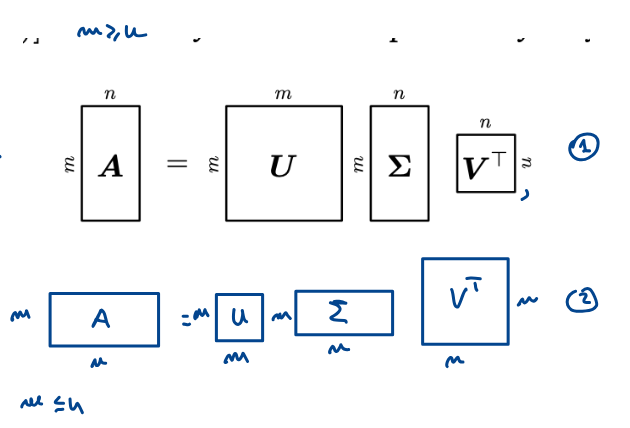
\includegraphics[width=0.588\textwidth]{img/svdpng.png}
    %\caption{}
\end{figure}
\vspace{2em}
\textbf{Teorema}: Sia $A$ la matrice ($m \times n$) con $k = rk(A) \, (\leq n \leq m)$ allora possiamo scrivere
\begin{align*}
    A = \sum_{i=1}^k \sigma_i u_i v_i^T
\end{align*}
Ovvero somma di matrici di rango 1.
\vspace{2em}\\
\begin{tcolorbox}[colback=blue!5!white, colframe=blue!75!black]
Gli autovalori $\lambda_i$ si possono calcolare per $A \in \mathbb{R}^{n \times n}$ con 
\begin{align*}
    det(A-\lambda I)=0
\end{align*}
Pero' questo si calcola solo se $A$ e' matrice quadrata!\\
Abbiamo sempre $n$ autovalori (inclusi i nulli).
\end{tcolorbox}
\textit{Ricorda}: $rk(A)=rk(A^TA)$.\\
Abbiamo la seguente relazione tra gli autovalori di $A^TA$ e i valori singolari di $A$:
\[
\begin{aligned}
A^T A & \\
&= (U \Sigma V^T)^T (U \Sigma V^T) \\
&= (V \Sigma^T U^T)(U \Sigma V^T) \\
&= V \Sigma^T \Sigma V^T \\
&= V \Sigma^2 V^T \\
&= V \begin{pmatrix}
        \sigma_1^2 & 0 & 0 \\
        0 & \sigma_2^2 & 0 \\
        0 & 0 & \sigma_n^2
    \end{pmatrix} V^T \\
\Rightarrow\ &\boxed{\sigma_j = \sqrt{\lambda_{i \text{ di } (A^T A)}}}
\end{aligned}
\]
$\Rightarrow$ abbiamo $rk(A)$ autovalori NON nulli e $n-rk(A)$ autovalori nulli!\\
\textit{Nota}: gli autovalori $\lambda_i$ di $A^TA$ possono essere in qualsiasi ordine; non c'è corrispondenza diretta tra l'indice $i$ di $\lambda_i$ e l'indice $i$ di $\sigma_i$.
\begin{itemize}
    \item $\sigma_1 = \sqrt{\lambda_{\max \text{ di } A^T A}} = \| A \|_2$ 
    \item $\sigma_n = \sqrt{\lambda_{\min \text{ di } A^T A}}=\| A^{-1} \|_2 \quad \rightarrow \| A^{-1} \| = \frac{1}{\sigma_n}$
    \item \hyperref[sec:cond]{$cond(A) = \frac{\sigma_1}{\sigma_n}$}
\end{itemize}
\vspace{2em}
Prendiamo ora in considereazione $A \in \mathbb{R}^{m \times n}, \, b \in \mathbb{R}^m, \, x \in \mathbb{R}^n$ 
\begin{align*}
    Ax = b
\end{align*}
Per Rouchè Capelli sappiamo che non ha soluzioni quindi
\begin{align*}
    Ax-b \neq 0
\end{align*}
definiamo $r$ il vettore \textbf{residuo}
\begin{align*}
    r = Ax-b
\end{align*}
Quindi piu' se $A$ sono i dati in input, $b$ output desiderato e $x$ quello che abbiamo imparato possiamo definire $r$ come errore del modello. \\
Nel capitolo \ref{sec:approssimazione} avevamo definito il problema dei minimi quadrati (lineare) come:
\begin{align*}
    \min_{\theta \in \mathbb{R}^k} \| \Phi \theta - y \|_2^2
\end{align*}
che nel caso del errore residuo $r$
\begin{align*}
    r = \min_x \| Ax - b \|_2^2
\end{align*}
Questo e' un problema \textbf{Linear Least Square}. \\
Come calcolare la soluzione? Sapendo che $r$ e' una funzione convessa:
\begin{itemize}
    \item $rk(A) = n = m$ $\Rightarrow$ 1 sola soluzione unica $\Rightarrow$ \hyperref[sec:met_grad]{gradiente} (iterativo), \hyperref[sec:min_quad]{equazioni normali} / Cholesky + LU oppure \hyperref[sec:svd]{SVD diretta}.
    \item $n \neq m$ e $b \not\in Im(A)$:
    \begin{itemize}
        \item nessuna soluzione esatta $\Rightarrow$ Trovare $\min_x \|Ax-b\|_2$: \hyperref[sec:met_grad]{gradiente} (iterativo) oppure \hyperref[sec:svd_pseudo]{SVD-pseudoinversa}.
    \end{itemize}
    \item $n \neq m$ e $b \in Im(A)$:
    \begin{itemize}
        \item Sovradeterminato ($m > n$): soluzione unica $\Rightarrow$ \hyperref[sec:met_grad]{gradiente} (iterativo), \hyperref[sec:min_quad]{equazioni normali} / Cholesky + LU, oppure \hyperref[sec:svd_pseudo]{SVD-pseudoinversa}.
        \item Sottodeterminato ($m < n$): infinite soluzioni compatibili $\Rightarrow$ \hyperref[sec:met_grad]{gradiente} (converge alla soluzione a norma euclidea minima) oppure \hyperref[sec:svd_pseudo]{SVD-pseudoinversa} (restituisce soluzione norma euclidea minima).
    \end{itemize}
\end{itemize}
\subsection*{Risoluzione di un problema LSQ con SVD}
\textbf{Forma sommatoria}: Abbiamo visto che possiamo trovare la soluzione per $rk(A) = n = m$
\begin{align*}
        Ax=b \\
        \Rightarrow U \Sigma V^T \hat{x}^* = b \\
        \Rightarrow \boxed{\hat{x}^*  = V \Sigma^{-1}U^T b}
\end{align*}
Costo computazionale: $O(\frac{4}{3}mn^2)$.\\
Ma se $m \neq n$ o anche se $rk(A) < n = m$ avremo dei $\sigma_{k+1} = 0$ che implica che $\not\exists \Sigma^{-1}$. \\
\vspace{1em}\\
Quindi come facciamo? \\
\textbf{Teorema pseudoinversa}: la soluzione $\hat{x}^*$ e' data ($r=rk(A)=n$):
\label{sec:svd_pseudo}
\begin{align*}
    \hat{x}^* = A^+b = V \Sigma^+ U^T b = \sum_{i=1}^r \frac{u_i^T b}{\sigma_i}v_i
\end{align*}
\begin{align*}
    \| \hat{x}^* \|_2^2 = \sum_{i=1}^r (\frac{u_i^T b}{\sigma_i}v_i)^2 \quad \| r^* \| = \sum_{i=r+1}^n (u_i^T b)^2
\end{align*}
\begin{tcolorbox}[colback=blue!5!white, colframe=blue!75!black]
Sia $A \in \mathbb{R}^{m\times n}$ con $rk(A) \leq min(m,n)$ e $A=U\Sigma V^T$. Si definisce \textbf{pseudoinversa}:
\begin{align*}
    A^+ = V \Sigma^+ U^T \\
    (\Sigma^+)_{ij}=\begin{cases}
        \frac{1}{\sigma_i} \text{ se } i=j \text{ e } i \leq k \\
        0 \text{ altrimenti} 
    \end{cases}
    = \begin{pmatrix}
            \frac{1}{\sigma_1} & 0 & 0 \\
            0 & \frac{1}{\sigma_2} & 0 \\
            0 & 0 & \frac{1}{\sigma_k}
        \end{pmatrix}
\end{align*}
Se $rk(A)=m=n \rightarrow A^+=A^{-1} \Rightarrow \Sigma^+ = \Sigma^{-1}$
\end{tcolorbox}
Costo computazionale: $O(\frac{4}{3}mn^2)$\\
\textbf{Definizione}: il numero di condizione in norma 2 di matrice $m \times n$ con valori singolari ($\sigma_1 > \dots > \sigma_k > \sigma_{k+1} = \dots = \sigma_n = 0$):
\label{sec:cond}
\begin{align*}
    \text{cond}(A) = \frac{\sigma_1}{\sigma_k}
\end{align*}
\begin{itemize}
    \item $cond(A) \approx 1$ matrice ben condizionata
    \begin{itemize}
        \item Piccoli errori nei dati $\to$ piccoli errori nel risultato
    \end{itemize}
    \item $cond(A) >> 1$ matrice mal condizionata
    \begin{itemize}
        \item Piccoli errori nei dati $\to$ grandi errori nel risultato
        \item Numericamente rischioso risolvere sistemi lineari $Ax=b$
    \end{itemize}
\end{itemize}
Possiamo utilizzare come indici per la precisione
\begin{itemize}
    \item Errore residuo: $Xa-y$
    \item MSE (mean square error): $media((x^* -x)^2)$
    \item $R^2$ (Coefficiente di determinazione), indica quanto il modello spiega la varianza dei dati: $1 - \frac{\sum_i (x^*_i - x_i)^2}{\sum_i (x_i - \bar{x})^2}$
\end{itemize}
\pagebreak
\section{Imaging e problemi inversi}
Data una immagine in scala di grigi possiamo definire la matrice $A$ come
\begin{align*}
    A[i][j] = \text{ intensita' del pixel}
\end{align*}
\subsection{Compressione SVD}
Possiamo rendere piu' efficiente una immagine attraverso la compressione:
\begin{align*}
    A \approx A_p = \sum_{i=1}^p u_i \cdot \sigma_i \cdot v_i^T
\end{align*}
con $p \leq rk(A)$. \\
Questo funziona perche $\sigma_k$ contiene piu' informazioni di $\sigma_{k+1}$. Quindi prendendo solo i primi $p$ valori singolari possiamo avere quasi tutte le informazioni pero' memorizziamo meno informazioni. \\
A livello teorico le due matrici contengono lo stesso numero di informazioni (NON GLI STESSI!!!), quindi salvandoli su disco il peso non dovrebbe variare. Pero' nei formati come \textit{png, jpeg, ecc.} ci sono delle compressioni interne gia' integrate e quindi grazie alla \textit{"pulizia"} del SVD otteniamo delle buone compressioni! \\
\vspace{1em}\\
Definiamo errore relativo
\begin{align*}
    E_r = \frac{\| A - A_p \|_2}{\|A\|_2}
\end{align*}
Definiamo fattore di compressione
\begin{align*}
    c_p = \frac{1}{p} \min(m,n)
\end{align*}
\subsection{Deblur}
Definiamo $x$ come l'immagine sorgente, possiamo dire che la funzione di blur (Point Spread Function (PSF)) e':
\begin{align*}
    A(x)
\end{align*}
ovvero
\begin{align*}
    A(x) = [K * x \mid P]
\end{align*}
con $K$ un kernel di convoluzione e $P$ il suo pattern di estensione. \\
\vspace{1px}\\
Ora definiamo $w$ come vettore di rumore (gaussiano), possiamo definire
\begin{align*}
    y^\delta = A(x) + w = [K * x \mid P] + w
\end{align*}
Quindi $y^\delta$ e' l'immagine con blur e rumore. \\
\textbf{Come otteniamo l'immagine originaria?}
Abbiamo $A$ come funzione di blur e $y^\delta$ come immagine distorta.
\begin{align*}
    \min_x \|Ax - y^\delta \|_2^2
\end{align*}
\begin{itemize}
    \item \hyperref[sec:min_quad]{Metodo dei minimi quadrati}: $A^T Ax=A^T y^\delta$ $\Rightarrow$ $O(mn^2 + n^3)$
    \item \hyperref[sec:svd]{SVD}: $O(\frac{4}{3}mn^2)$
    \item Metodo dei minini quadrati con \hyperref[sec:cgls]{\textbf{CGLS}}: $\approx O(k \cdot mn)$ con $k \in \mathbb{R}$
\end{itemize}
Definiamo l'errore relativo
\begin{align*}
    E_r = \frac{\| x_\text{originale} - x \|_2^2}{\| x_\text{originale} \|_2^2}
\end{align*}
\subsection*{Regolarizzazione di Tikhonov}
Possiamo ulteriormente migliorare il deblur attraverso la regolarizzazione del rumore. \\
Partiamo da $y^\delta = Ax+w$, definiamo la regolarizzazione
\begin{align*}
    x_\lambda = \text{arg} \min_x \| Ax - y^\delta \|_2^2 + \lambda^2 \| x \|_2^2
\end{align*}
Dove 
\begin{itemize}
    \item $\| Ax - y^\delta \|_2^2$ indica la fedelta' sulla immagine originale (fit dei dati)
    \item $\lambda^2 \| x \|_2^2$ indica la complessità della soluzione, ovvero quanto dobbiamo limitare la "rumorosita'" della soluzione (regolarizzazione)
\end{itemize}
Questo e' \textbf{Tikhonov 1-ordine}, serve quando abbiamo $A(x)$ mal condizionata quindi con piccole variazioni abbiamo grandi sbalzi, con il $1-ordine$ possiamo regolarizzare e ottenere una soluzione stabile con picchi rumorosi ridotti. \\
Dobbiamo risolvere la funzione
\begin{align*}
    \Rightarrow f(x) = \| Ax - y^\delta \|_2^2 + \lambda^2 \| x \|_2^2 \\
    \Rightarrow f(x) = (Ax - y^\delta)^T(Ax - y^\delta)+(\lambda^2 \| x \|_2^2 )^T(\lambda^2 \| x \|_2^2 )
\end{align*}
e dato che minimizziamo cerchiamo la $x$ minima ovvero $x | \nabla f(x)=0$:
\begin{align*}
    \frac{d}{dx}[(Ax - y^\delta)^T(Ax - y^\delta)+(\lambda^2 \| x \|_2^2 )^T(\lambda^2 \| x \|_2^2 )] = 0\\
    \Rightarrow (A^TA + \lambda^2)x = A^T y^\delta
\end{align*}
Ora possiamo scelgiere il nostro metodo preferito per risolvere la SPD.\\
\vspace{2em}\\
\textbf{Ma come scegliamo il parametro di regolarizzazione $\lambda$?}\\
Teoricamente possiamo definirlo come 
\begin{align*}
    x_{opt} = \min_\lambda \|x_\lambda - x_{GT} \|_2
\end{align*}
Questo vuol dire minimizzare l'errore assoluto, sarebbe la cosa migliore da fare ma implica conoscere $x_{GT}$ che nella realta' e' impossibile. \\
E come lo calcoliamo senza sapere $x_{GT}$? Un metodo e' il \textbf{principio di massima discrepanza}:
\begin{align*}
    \| Ax_\lambda - y^\delta \|_2 \approx \|w\|_2 \\
    \Rightarrow \lambda_{DP} = \text{arg} \min_{\lambda} | \|A(x_\lambda) - y^\delta \|_2 - \|w\|_2  |
\end{align*}
Generalmente siamo su $\lambda_{DP} \approx 0.01$. \\
Questo pero richiede che conosciamo il rumore $w$, pero' normalmente non e' noto. \\
Per la valutazione del risultato ottenuto facciamo
\begin{align*}
    E_r = \frac{\| x_{GT} - x_{tikhonov} \|_2^2}{\| x_{GT} \|_2^2}
\end{align*}
\subsection*{Regolarizzazione con variazione totale}
Un altro metodo di regolarizzazione molto utilizzato e'
\begin{align*}
    TV(x) = \| \nabla x \|_1
\end{align*}
Ma dato che non e' differenziabile in (0,0) aggiungiamo un piccolo $\beta$:
\begin{align*}
    TV_\beta(x) = \sum_{i,j} \sqrt{ (\nabla x_{i,j})^2 + \beta^2 }
\end{align*}
Quindi dobbiamo risolvere 
\begin{align*}
    \min_x \| Ax - y^\delta \|_2^2 + \lambda TV_\beta (x)
\end{align*}
Il valore $\lambda$ come lo scegliamo? A valore fisso, oppure con metodi iterativi (anche DP). \\
Questo puo' essere risolto con il \hyperref[sec:met_grad]{metodo del gradiente + backtracking}. 
\begin{algorithm}[H]
\caption{TV + Discrepancy Principle con risoluzione via GD + regolarizzazione}
\begin{algorithmic}[1]
\State $\lambda_\text{list} = [\dots]$
\State soluzioni[]
\State residui[]
\For{$\lambda$ in $\lambda_{\text{list}}$}
    \State x, \text{alpha}, \text{storico\_iterazioni}, \text{n-iter} = \text{GD\_REG}($A,   y^\delta, n=1.0, p=1, \text{reg}=\lambda, TV()_\beta,q=1$)
    \State soluzioni.append($x$)
    \State residui.append($\|A x - y^\delta\|_2^2$)
\EndFor

\State ${idx}_\text{DP} = \text{index}(\min(residui - w), residui)$
\State $\lambda_{\text{DP}} = \lambda_{\text{list}}[idx_{\text{DP}}]$
\State $x_{\text{final}} = \text{soluzioni}[idx_{\text{DP}}]$

\end{algorithmic}
\end{algorithm}

\end{document}